\documentclass[tikz]{standalone}
\usetikzlibrary{arrows, calc, positioning}
\begin{document}
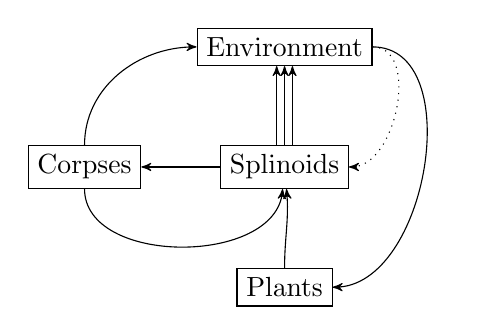
\begin{tikzpicture}[>=stealth',
  every node/.style={draw}
 ]
 \node (E) {Environment};
 \node [below=of E] (S) {Splinoids};
 \node [left=of S] (C) {Corpses};
 \node [below=of S] (P) {Plants};
 
 \draw [->, dotted] (E.east) to [out=0, in=0] (S);
 \draw [->] (E.east) to [out=0, in=0] (P);
 \draw [->] (S) to (C);
 \draw [->] (C.north) to [out=90, in=180] (E);
 \draw [->] (C.south) to [out=270, in=265] (S);
 \draw [->] (P) to [out=90, in=275] (S);
 
 \foreach \x in {-1,0,1} {
  \def\dx{.1}
  \draw [->] ($(S.north)+(\dx*\x,0)$) -- ($(E.south)+(\dx*\x,0)$);
 }
\end{tikzpicture}

%    Plant min energy: 12.5664
% Splinoid min energy: 0.0628319
%    Old age duration: 327.114, 117.329, 71.4845
% Starvation duration:
% 	10.2766, 3.686, 2.24575
% 	256.915, 92.15, 56.1438
	
\end{document}
